\let\lesson\undefined
\newcommand{\lesson}{\phantomlesson{Bài 17.}}
\let\lesson\undefined
\newcommand{\lesson}{\phantomlesson{Bài 17.}}


\setcounter{section}{2}
\section{Trắc nghiệm}
\Opensolutionfile{ans}[ans/VN12-Y24-PH-SYL-031P-TN]
\setcounter{ex}{0}
% ===================================================================
\begin{ex}\mkstar{1}
	Chỉ ra phát biểu \textbf{sai} khi nói về hiện tượng phóng xạ.
	\choice
	{Hiện tượng phóng xạ là hiện tượng một hạt nhân không bền vững tự phát phân rã, phát ra các tia phóng xạ và biến đổi thành hạt nhân khác}
	{\True Hiện tượng phóng xạ chịu ảnh hưởng bởi các yếu tố bên ngoài như nhiệt độ, áp suất, $\dots$}
	{Có 3 loại phóng xạ là phóng xạ $\alpha, \beta$ và $\gamma$; trong đó phóng xạ $\beta$ được chia làm hai loại là phóng xạ $\beta^-$ và phóng xạ $\beta^{+}$}
	{Do tia $\gamma$ có bản chất là sóng điện từ nên phóng xạ $\gamma$ không đi kèm với việc biến đổi hạt nhân mẹ thành hạt nhân khác}
	\loigiai{

	}
\end{ex}
% ===================================================================
\begin{ex}\mkstar{1}
	Trong các định luật bảo toàn sau:
	\begin{enumerate}[label=(\arabic*)]
		\item Bảo toàn động lượng.
		\item Bảo toàn số khối.
		\item Bảo toàn khối lượng.
		\item Bảo toàn năng lượng toàn phần.
		\item Bảo toàn số proton.
	\end{enumerate}
	Hiện tượng phóng xạ tuân theo bao nhiêu định luật bảo toàn?
	\choice
	{2}
	{\True 3}
	{4}
	{5}
	\loigiai{
	Chọn (1); (2); (4).
	}
\end{ex}
% ===================================================================
\begin{ex}\mkstar{1}
	Tìm phát biểu \textbf{sai}.
	\choice
	{Hạt $\beta^{-}$ là hạt electron}
	{Tia $\beta^{-}$ có khả năng ion hoá môi trường}
	{Trong điện trường giữa hai bản tụ điện, tia $\beta^{-}$bị lệch về phía bản mang điện dương của tụ điện}
	{\True Tia $\beta^{-}$có tầm bay ngắn hơn tia $\alpha$}
	\loigiai{}
\end{ex}
% ===================================================================
\begin{ex}\mkstar{1}
Tìm phát biểu \textbf{sai}.
	\choice
	{Tia $\beta^{+}$có tầm bay xa hơn tia $\alpha$}
	{Hạt $\beta^{+}$có cùng khối lượng với electron nhưng mang điện tích nguyên tố dương}
	{Tia $\beta^{+}$ cũng làm ion hoá môi trường nhưng yếu hơn tia $\alpha$}
	{\True Tia $\beta^{+}$ bị lệch về phía bản mang điện dương của tụ điện khi đi qua điện trường giữa hai bản tụ điện}
	\loigiai{}
\end{ex}
% ===================================================================
\begin{ex}\mkstar{1}
	Công thức nào dưới đây \textbf{đúng} với nội dung của định luật phóng xạ?
	\choice
	{$m=m_0e^{\lambda t}$}
	{\True $m=m_0e^{-\lambda t}$}
	{$m=m_0 e^{-\frac{\lambda}{t}}$}
	{$m=m_0 e^{-\frac{1}{T}}$}
	\loigiai{}
\end{ex}
% ===================================================================
\begin{ex}\mkstar{1}
	Trong một mẫu chất phóng xạ, tại thời điểm ban đầu $(t=0)$, mẫu chất có $N_0$ hạt nhân. Biết hằng số phóng xạ và chu kì bán rã của chất phóng xạ này lần lượt là $\lambda$ và $T$. Sau đó một khoảng thời gian $\Delta t$, số lượng hạt nhân còn lại trong mẫu chất đó được xác định bằng biểu thức nào sau đây?
	\choice
	{$N_{t}=N_0 e^{\lambda \Delta t}$}
	{$N_{t}=N_0 2^{\frac{\Delta t}{T}}$}
	{\True $N_{t}=N_0 e^{-2 \Delta t}$}
	{$N_{t}=N_0 2^{-\Delta t}$}
	\loigiai{}
\end{ex}
% ===================================================================
\begin{ex}\mkstar{2}
	Trong các phát biểu sau khi nói về hiện tượng phóng xạ, có bao nhiêu phát biểu \textbf{đúng}?
	\begin{enumerate}[label=(\arabic*)]
		\item Chu kì bán rã là thời gian để một nửa số hạt nhân ban đầu bị phân rã.
		\item Mối quan hệ giữa chu kì bán rã và hằng số phóng xạ là $\lambda=T \cdot \ln 2$.
		\item Trong hiện tương phóng xạ, tia $\gamma$ thường sẽ phát kèm theo các tia $\alpha$ và $\beta$.
		\item Độ phóng xạ là đại lượng đặc trưng cho tính phóng xạ mạnh hay yếu của một lượng chất phóng xạ.
		\item Trong hiện tượng phóng xạ, độ phóng xạ tăng dần theo thời gian với quy luật hàm số mũ.
	\end{enumerate}
	\choice
	{1}
	{2}
	{\True 3}
	{4}
	\loigiai{Chọn phát biểu: 1; 3 và 4.}
\end{ex}
% ===================================================================
\begin{ex}\mkstar{2}
	Chiếu 3 chùm tia thu được từ quá trình phóng xạ hạt nhân lần lượt qua tấm giấy, nhôm và chì như hình bên. Các tia 1, tia 2, tia 3 theo thứ lần lượt là
	\begin{center}
		\includegraphics[width=0.4\linewidth]{../figs/VN12-Y24-PH-SYL-031P-2}
	\end{center}
	\choice
	{tia $\beta$, tia $\alpha$, tia $\gamma$}
	{\True tia $\alpha$, tia $\beta$, tia $\gamma$}
	{tia $\beta$, tia $\gamma$, tia $\alpha$}
	{tia $\gamma$, tia $\alpha$, tia $\beta$}
	\loigiai{}
\end{ex}
% ===================================================================
\begin{ex}\mkstar{2}
	Bắn chùm tia phóng xạ qua không gian có từ trường đều như hình vẽ. Chùm tia A là 	
	\begin{center}
		\includegraphics[width=0.2\linewidth]{../figs/VN12-Y24-PH-SYL-031P-1}
	\end{center}
	\choice
	{\True tia $\gamma$}
	{tia $\alpha$}
	{tia $\beta^+$}
	{tia $\beta^-$}
	\loigiai{
		Chùm gamma không mang điện tích nên không bị lệch phương trong từ trường.	
	}
\end{ex}
% ===================================================================
\begin{ex}\mkstar{2}
	Bắn chùm tia phóng xạ qua không gian có từ trường đều như hình vẽ. Chùm tia C là 	
		\begin{center}
		\includegraphics[width=0.2\linewidth]{../figs/VN12-Y24-PH-SYL-031P-1}
	\end{center}
	\choice
	{tia $\gamma$}
	{tia $\alpha$}
	{tia $\beta^+$}
	{\True tia $\beta^-$}
	\loigiai{
		Chùm tia $\beta^-$ mang là chùm $e^-$ mang điện tích âm, áp dụng quy tắc bàn tay trái, lực từ tác dụng lên $e^-$ làm nó lệch hướng cùng chiều quay của kim đồng hồ.
	}
\end{ex}
% ===================================================================
\begin{ex}\mkstar{2}
	Chùm tia $\alpha$ và $\beta^-$ được bắn ra với cùng động năng phi tương đối tính. Tỉ số giữa mỗi hạt trong 2 chùm tia là
	\choice
	{\True $\dfrac{v_\beta}{v_\alpha}=85,73$}
	{$\dfrac{v_\beta}{v_\alpha}=2$}
	{$\dfrac{v_\beta}{v_\alpha}=60,6$}
	{$\dfrac{v_\beta}{v_\alpha}=4$}
	\loigiai{
		$$K_\alpha=K_\beta\Leftrightarrow \dfrac{1}{2}m_\alpha v^2_\alpha=\dfrac{1}{2}m_\beta v^2_\beta$$
		$$\Rightarrow \dfrac{v_\beta}{v_\alpha}=\sqrt{\dfrac{m_\alpha}{m_\beta}}=\sqrt{\dfrac{4m_p}{m_e}}\approx 85,7.$$
	}
\end{ex}
% ===================================================================
\begin{ex}\mkstar{3}
	Một mẫu phóng xạ có chu kì bán rã là 3 ngày. Sau 9 ngày, khối lượng của mẫu phóng xạ này còn lại là $\SI{2}{\kilogram}$. Khối lượng ban đầu của mẫu là bao nhiêu?
	\choice
	{$\SI{15}{\kilogram}$}
	{\True $\SI{16}{\kilogram}$}
	{$\SI{17}{\kilogram}$}
	{$\SI{14}{\kilogram}$}
	\loigiai{
	
	}
\end{ex}
% ===================================================================
\begin{ex}\mkstar{3}
	$\ce{_{84}^{210}Po}$ là một đồng vị phóng xạ có chu kì bán rã là 138,4 ngày. Xét một mẫu chất đang chứa $N_0$ hạt nhân $\ce{_{84}^{210}Po}$ (tại thời điểm ban đầu). Sau bao lâu kể từ thời điểm ban đầu thì tỉ số giữa số hạt nhân $\ce{_{84}^{210}Po}$ đã phân rã thành hạt nhân khác và số hạt nhân $\ce{_{84}^{210}Po}$ còn lại bằng 7 ?
	\choice
	{\True 415,2 ngày}
	{387,5 ngày}
	{34,6 ngày}
	{968,8 ngày}
	\loigiai{Khoảng thời gian cần tìm là:
		$$
		\frac{\Delta N_{t}}{N_{t}}=\frac{N_0\left(1-2^{-\frac{t}{T}}\right)}{N_0 2^{-\frac{t}{T}}}=2^{\frac{t}{T}}-1=7 \Rightarrow t=3 T=3\cdot138,4=\SI{415.2}{\text{ngày}}.
		$$}
\end{ex}
% ===================================================================
\begin{ex}\mkstar{3}
	Chu kì bán rã của một mẫu phóng xạ là 6 giờ. Lúc đầu mẫu có khối lượng $\SI{2.4E-2}{\kilogram}$. Hỏi sau một ngày đêm, khối lượng của mẫu còn lại bằng bao nhiêu?
	\choice
	{$\SI{3E-3}{\kilogram}$}
	{\True $\SI{1.5E-3}{\kilogram}$}
	{$\SI{2.5E-3}{\kilogram}$}
	{$\SI{2E-3}{\kilogram}$}
	\loigiai{}
\end{ex}
% ===================================================================
\begin{ex}\mkstar{3}
	Sau 3 giờ phóng xạ, số hạt nhân của một mẫu đồng vị phóng xạ chỉ còn $\SI{25}{\percent}$ số hạt nhân ban đầu. Chu kì bán rã của đồng vị này là
	\choice
	{1 giờ}
	{2 giờ}
	{2,5 giờ}
	{\True 1,5 giờ}
	\loigiai{}
\end{ex}
% ===================================================================
\begin{ex}\mkstar{3}
	Một mẫu chất phóng xạ $X$ phân rã theo thời gian và phát ra các hạt $\alpha$. Số lượng các hạt $\alpha$ này được ghi nhận bởi một máy thu (ống Geiger-Muller) và được biểu diễn theo thời gian $t$ như đồ thị ở hình bên.
\begin{center}
		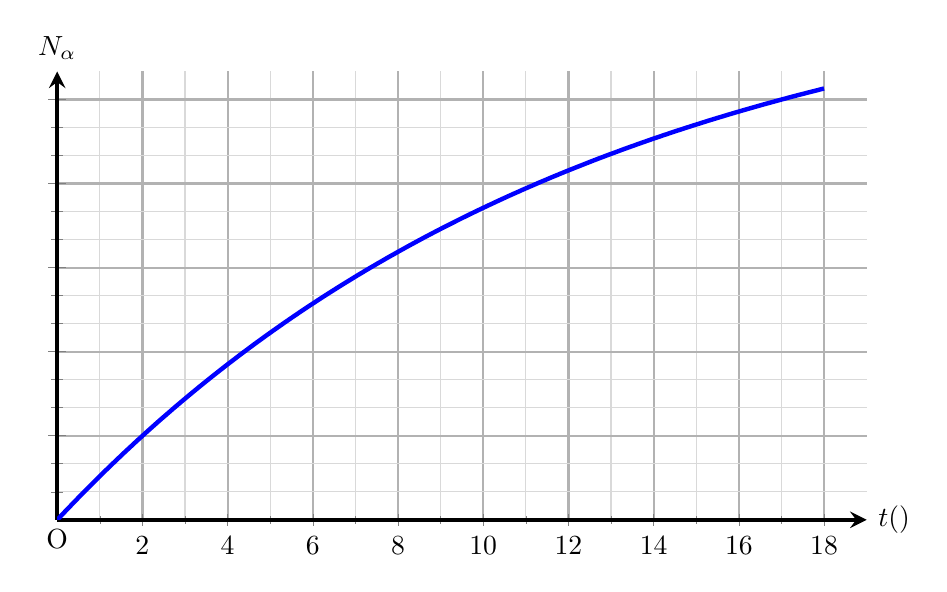
\begin{tikzpicture}  
		\begin{axis}[  ultra thick,
			xmin=0,  
			xmax=19,  
			xtick={0,2,...,18},
			ytick={0,3,...,15},
			minor x tick num=1,
			minor y tick num=2,
			ymin=0,  
			ymax=16, 
			samples=300,
			yticklabels=\empty,
			axis lines=center, 
			grid style={step=1, line width =0.4pt, color=gray!30!white},
			grid=both, %giới hạn ô lưới
			major grid style={line width=0.8pt,gray!60!white},
			xlabel=$\xsi{t}{\left(\si{\second}\right)}$, 		ylabel=$N_{\alpha}$,
			every axis y label/.style={at=(current axis.above origin),anchor=south},  
			every axis x label/.style={at=(current axis.right of origin),anchor=west}, xscale=1.5 ]
			\addplot [ultra thick, blue, smooth, domain=0:18] {20.0647*(1-2^(-x/8.56))};  
		\end{axis}  
		\node[below] at (0,0) {O};
	\end{tikzpicture}
\end{center}
	Hằng số phóng xạ của chất phóng xạ là
	\choice
	{\True $\SI{0.081}{\second^{-1}}$}
	{$\SI{0.173}{\second^{-1}}$}
	{$\SI{0.231}{\second^{-1}}$}
	{$\SI{0.058}{\second^{-1}}$}
	\loigiai{
	$$
	\begin{aligned}
		& N_\alpha=N_0 \cdot\left(1-2^{-\frac{t}{T}}\right) \Rightarrow
		\begin{cases}
			3=N_0 \cdot\left(1-2^{-\frac{2}{T}}\right) \\
			15=N_0 \cdot\left(1-2^{-\frac{17}{T}}\right)
		\end{cases}
		\Rightarrow \frac{3}{15}=\frac{1-2^{-\frac{2}{T}}}{1-2^{-\frac{17}{T}}} \Rightarrow T \approx \SI{8.56}{\second} \\
		& \Rightarrow \lambda=\frac{\ln 2}{T}=\frac{\ln 2}{8,56} \approx \SI{0.081}{\second^{-1}}.
	\end{aligned}
	$$
	}
\end{ex}
% ===================================================================
\begin{ex}\mkstar{4}
	Tỉ lệ uranium hiện tại trong tự nhiên là $\SI{0.72}{\percent}\ \ce{^{235}U}$ và $\SI{99.27}{\percent}\ \ce{^{238}U}$. Tỉ lệ phần trăm của $\ce{^{235}U}$ trong tự nhiên sẽ là bao nhiêu nếu ở thời điểm Trái Đất được hình thành (cách nay 4,5 tỉ năm)? Biết rằng chu kì bán rã của $\ce{^{235}U}$ là 704 triệu năm và của $\cee{^{238}U}$ là 4,47 tỉ năm.
	\choice
	{$\SI{26.73}{\percent}$}
	{\True $\SI{23.26}{\percent}$}
	{$\SI{99.98}{\percent}$}
	{$\SI{98.56}{\percent}$}
	\loigiai{
		Gọi $a$ là tỉ lệ phần trăm $\ce{^{235}U}$ ban đầu trong tự nhiên và $N_0$ là tổng số hạt uranium khi Trái Đất mới hình thành.
		\begin{center}
			\begin{tabular}{|C{4cm}|C{5cm}|C{5cm}|}
				\hline
				\textbf{Đồng vị}&\textbf{Ban đầu}& \textbf{Hiện tại}\\
				\hline
				$\ce{^{235}U}$ & $a\cdot N_0$ & $a\cdot N_0\cdot 2^{-\dfrac{t}{T_{235}}}$\\
				\hline
				$\ce{^{238}U}$ & $\left(1-a\right)\cdot N_0$ & $\left(1-a\right)\cdot N_0\cdot 2^{-\dfrac{t}{T_{238}}}$\\
				\hline
			\end{tabular}
		\end{center}	
		Ta có:
		$$\si{\percent}\ce{^{235}U}=\dfrac{N_{\ce{^{235}U}}}{N_{\ce{^{235}U}+N_{\ce{^{238}U} }}}=\dfrac{a\cdot2^{-\dfrac{t}{T_{235}}}}{a\cdot2^{-\dfrac{t}{T_{235}}}+\left(1-a\right)\cdot2^{-\dfrac{t}{T_{238}}}}$$
		$$\Leftrightarrow\SI{0.72}{\percent}=\dfrac{a\cdot2^{-\dfrac{4,5}{\SI{704E-3}{}}}}{a\cdot2^{-\dfrac{4,5}{\SI{704E-3}{}}}+\left(1-a\right)\cdot2^{-\dfrac{4,5}{4,47}}}\Rightarrow a=\SI{23.26}{\percent}.$$
	}
\end{ex}
\Closesolutionfile{ans}
\section{Trắc nghiệm đúng/sai}
\Opensolutionfile{ans}[ans/VN12-Y24-PH-SYL-031P-TF]
\setcounter{ex}{0}

% ===================================================================
\begin{ex}\mkstar{2}
	$\ce{_{92}^{238}U}$ là một đồng vị phóng xạ có hằng số phóng xạ bằng $\SI{4.916E-18}{\second^{-1}}$. Biết rằng sau một khoảng thời gian nào đó, $\ce{_{92}^{238}U}$ xảy ra phóng xạ $\alpha$ và biến đổi thành hạt nhân con $\ce{X }$. Trong mỗi phát biểu sau, em hãy chọn đúng hoặc sai.
	\choiceTF[t]
	{\True Quá trình phóng xạ của $\ce{_{92}^{238}U}$ là một phản ứng hạt nhân toả năng lượng}
	{Hạt nhân con $\ce{X}$ được tạo thành từ quá trình phóng xạ trên là $\ce{_{92}^{234}U}$}
	{\True Chu kì bán rã của $\ce{_{92}^{238}U}$ là $\SI{1.41E17}{\second}$ (làm tròn đến 2 chữ số thập phân sau dấu phẩy)}
	{Xét một mẫu chất tại thời điểm ban đầu chứa $\SI{0.1}{\gram}$ đồng vị phóng xạ $\ce{_{92}^{238}U}$. Sau 100 triệu năm (xem như mỗi năm có 365 ngày), khối lượng $\ce{_{92}^{238}U}$ còn lại trong mẫu chất đó khoảng $\SI{0.089}{\gram}$}
	\loigiai{}
\end{ex}
% ===================================================================
\begin{ex}\mkstar{2}
	Máy chiếu xạ sử dụng nguồn phóng xạ $\beta^{-}$ cobalt $\ce{_{27}^{60}Co}$ với chu kì bán rã 5,27 năm để điều trị ung thư. Nguồn phóng xạ trong máy sẽ cần được thay mới nếu như độ phóng xạ của nó giảm còn bằng $\SI{50}{\percent}$ độ phóng xạ ban đầu. Các phát biểu dưới đây là đúng hay sai?
	\choiceTF[t]
	{Sản phẩm phân rã của cobalt $\ce{_{27}^{60}Co}$ là nickel $\ce{_{28}^{61}Ni}$}
	{Hằng số phóng xạ của cobalt $\ce{_{27}^{60}Co}$ là $\SI{0.132}{\second^{-1}}$}
	{\True Nguồn phóng xạ của máy cần được thay thế sau mỗi 5,27 năm}
	{\True Tại thời điểm thay nguồn phóng xạ, số hạt nhân $\ce{_{27}^{60}Co}$ còn lại trong nguồn bằng $\SI{50}{\percent}$ số hạt nhân $\ce{_{27}^{60}Co}$ ban đầu}
	\loigiai{}
\end{ex}
% ===================================================================
\begin{ex}\mkstar{3}
	Hình bên biểu diễn sự phụ thuộc của số hạt còn lại và số hạt đã bị phân rã theo thời gian $t$ của một mẫu chất phóng xạ.
	\begin{center}
		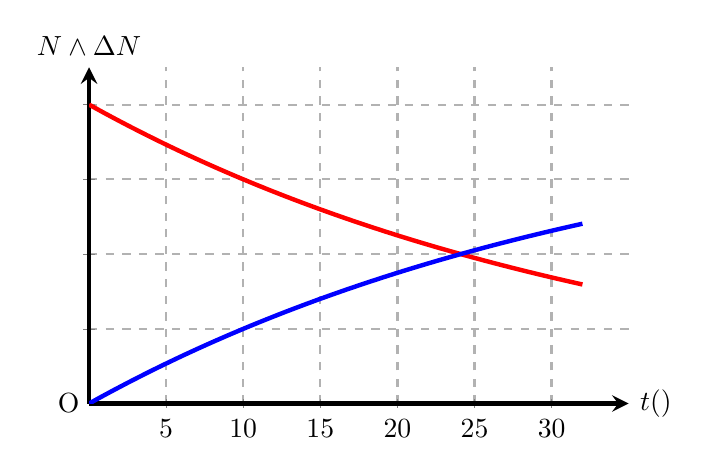
\begin{tikzpicture}  
			\begin{axis}[  ultra thick,yscale=0.75,
				xmin=0,  
				xmax=35,  
				xtick={0,5,...,30},
				ytick={0,1,...,5},
				yticklabels=\empty,
				minor x tick num=0,
				minor y tick num=0,
				ymin=0,  
				ymax=4.5, 
				samples=300,
				axis lines=middle, 
				grid style={step=1, line width =0.4pt, color=gray!30!white},
				grid=both,
				major grid style={line width=0.8pt,gray!60!white, dashed},
				xlabel=$\xsi{t}{\left(\si{\hour}\right)}$, 		ylabel=$N\wedge\Delta N$,
				every axis y label/.style={at=(current axis.above origin),anchor=south},  
				every axis x label/.style={at=(current axis.right of origin),anchor=west},  ]
				\addplot [ultra thick, red, smooth, domain=0:32] {4*2^(-x/24.094)};  
				\addplot [ultra thick, blue, smooth, domain=0:32] {4-4*2^(-x/24.094)};
			\end{axis}  
			
			\node[left] at (0,0) {O};
		\end{tikzpicture}
		
	\end{center}	
	\choiceTF[t]
	{Tại thời điểm $\SI{10}{\hour}$, số hạt bị phân rã gấp 3 lần số hạt còn lại}
	{Chu kì bán rã của mẫu chất là $\SI{25}{\hour}$}
	{\True Tại thời điểm $\SI{30}{\hour}$, số hạt nhân phóng xạ đã giảm 2,37 lần so với ban đầu}
	{Nếu tăng áp suất trong phóng, quá trình phòng xạ của mẫu chất sẽ diễn ra nhanh hơn}
	\loigiai{
		\begin{itemchoice}
			\itemch Sai. Tại thời điểm $\SI{10}{\hour}$, số hạt còn lại gấp 3 lần số hạt bị phân rã.
			\itemch Sai. Chu kì bán rã của mẫu chất là $T\approx\SI{24.09}{\hour}$.\\
			Tại thời điểm $t=\SI{10}{\hour}$ thì $N=\dfrac{3}{4}N_0$ nên:
			$$2^{-\dfrac{10}{T}}=\dfrac{3}{4}\Rightarrow T\approx\SI{24.09}{\hour}.$$
			\itemch Đúng. Tại thời điểm $t=\SI{30}{\hour}$ thì số hạt còn lại
			$$N=\dfrac{N_0}{2^{\dfrac{t}{T}}}=\dfrac{N_0}{2^{\dfrac{30}{24,09}}}\approx\dfrac{N_0}{2,37}.$$
			\itemch Sai. Quá trình phóng xạ không phụ thuộc điều kiện bên ngoài.
		\end{itemchoice}	
	}
\end{ex}

\Closesolutionfile{ans}
\section{Tự luận}
\Opensolutionfile{ans}[ans/VN12-Y24-PH-SYL-031P-TL]
\setcounter{ex}{0}
% ======================================================================
\begin{ex}\mkstar{2}
	 Cho một mẫu chất đang chứa $N_0$ hạt nhân với chu kì bán rã $T$ vào thời điểm ban đầu $\left(t_0=0\right)$. Tính số hạt nhân đã phóng xạ tại thời điểm $t=2 T$.
	\loigiai{
	$\Delta N=N_0-N_t=N_0\left(1-2^{-\dfrac{t}{T}}\right)=\dfrac{3}{4}N_0.$
	}
\end{ex}
% ======================================================================
\begin{ex}\mkstar{2}
	Xác định giá trị của số khối $A$ và số hiệu nguyên tử $Z$ trong các phương trình phóng xạ sau:
	\begin{enumerate}[label=\alph*), parsep=0.25cm]
		\item $\ce{_{83}^{212}Bi} \longrightarrow\ce{_Z^{A}X}+\ce{_2^4He}$.
		\item $\ce{_{90}^{234}Th} \longrightarrow\ce{_{88}^{230}Ra}+\ce{^A_ZX}$.
		\item $\ce{_{84}^{210}Po} \longrightarrow \ce{^A_ZX}+\alpha$.
		\item $\ce{_5^{12}B} \longrightarrow\ce{^A_ZX}+\beta+\bar{v}_{e}$.
	\end{enumerate}
	\loigiai{
	\begin{enumerate}[label=\alph*)]
		\item $A=208; Z=81$.
		\item $A=4; Z=2$.
		\item $A=206; Z=82$.
		\item $A=12; Z=6$.
	\end{enumerate}
	}
\end{ex}
% ======================================================================
\begin{ex}\mkstar{2}
	Trên thực tế, nếu một hạt nhân không bền phóng xạ tạo thành hạt nhân mới. Hạt nhân mới cũng không bền tiếp tục phân rã nhiều lần đến khi tạo thành một hạt nhân bền thì quá trình này sẽ dừng lại. Tập hợp các hạt nhân từ hạt nhân không bền đầu tiên đến hạt nhân bền cuối cùng được gọi là một họ phóng xạ. Xét sự phóng xạ của họ phóng xạ thorium (bắt đầu với $\ce{_{90}^{232}Th}$ và kết thúc tại $\ce{_{82}^{208}Pb}$) với phương trình phóng xạ thu gọn như sau:
	$$\ce{_{90}^{232}Th} \longrightarrow\ce{_{82}^{208}Pb}+x \beta+y \alpha.
	$$
	Hãy xác định giá trị của $x$ và $y$.
	\loigiai{
	Dựa trên định luật bảo toàn điện tích và bảo toàn số nucleon, ta lập được hệ phương trình sau:
	$$\begin{cases}
		232=208+4y\\
		90=82-x+2y
	\end{cases}\Rightarrow \begin{cases}
	y=6\\
	x=4
	\end{cases}.$$
	}
\end{ex}

% ======================================================================
\begin{ex}\mkstar{2}
	Một mẫu than bùn khi được đem lên từ vùng đầm lầy cổ có chứa $\SI{980}{\micro\gram}$ đồng vị phóng xạ $\ce{_6^{14}C}$. Biết rằng chu kì bán rã của $\ce{_6^{14}C}$ là 5730 năm. Hãy xác định:
	\begin{enumerate}[label=\alph*)]
		\item khối lượng $\ce{_6^{14}C}$ chứa trong mẫu than bùn này sau 2000 năm.
		\item thời điểm tại đó khối lượng $\ce{_6^{14}C}$ trong mẫu than bùn này còn lại $\SI{100}{\gram}$.
	\end{enumerate}
	\loigiai{
	\begin{enumerate}[label=\alph*)]
		\item Khối lượng $\ce{_6^{14}C}$ chứa trong mẫu than bùn sau 2000 năm là:
		$$
		m_{{t}}=m_0 2^{-\frac{t}{T}}=980\cdot2^{-\frac{2000}{5730}} \approx \SI{769.4}{\micro\gram}.
		$$
		\item Thời điểm mà khối lượng $\ce{_6^{14}C}$ trong mẫu than bùn này còn lại $\SI{100}{\micro\gram}$ là:
		$$
		m_{t}=m_0 2^{-\frac{t}{T}} \Rightarrow t=-T \log _2\left(\frac{m_{t}}{m_0}\right)=-5730 \cdot \log _2\left(\frac{100}{980}\right) \approx \SI{18867.64}{\text{năm}}.
		$$
	\end{enumerate}
	}
\end{ex}
% ======================================================================
\begin{ex}\mkstar{3}
	Xét đồng vị không bền của nickel là $\ce{_{28}^{66}Ni}$ phát ra tia phóng xạ $\beta$ và biến thành hạt nhân con $\ce{_{29}^{66}Cu}$. Biết rằng khối lượng của các hạt nhân trên lần lượt là $m_{\ce{Ni}}=\SI{65.9291}{amu}$ và $m_{\ce{Cu}}=\SI{65.9289}{amu}$; năng lượng toả ra của quá trình phóng xạ được xác định bởi biểu thức $\Delta E=\left(m_1-m_2\right) c^2$ với $m_1$ và $m_2$ lần lượt là tổng khối lượng của các hạt trước và sau phản ứng.
	\begin{enumerate}[label=\alph*)]
		\item Viết phương trình phân rã của $\ce{_{28}^{66}Ni}$.
		\item Tính năng lượng toả ra của quá trình phóng xạ nói trên.
	\end{enumerate}
	\loigiai{
	\begin{enumerate}[label=\alph*)]
		\item $\ce{_{28}^{66}Ni} \longrightarrow\ce{_{-1}^0e}+ \ce{_{29}^{66}Cu}$.
		\item Vì khối lượng của electron là không đáng kể nên năng lượng toả ra của quá trình phóng xạ là:
		$$
		\Delta E=\left(m_{\ce{Ni}}-m_{\ce{Cu}}\right) c^2=(65,9291-65,9289) \cdot 931,5=\SI{0.1863}{\mega\electronvolt}.
		$$
	\end{enumerate}
	}
\end{ex}

% ======================================================================
\begin{ex}\mkstar{3}
	Một trong những ứng dụng rộng rãi của hiện tượng phóng xạ là xác định niên đại của cổ vật bằng phương pháp $\ce{^14}C$. Trường hợp xác định niên đại nổi tiếng bằng phương pháp $\ce{^14}C$  là sự kiện liên quan đến tấm vải liệm Turin (một tấm vải dài được cho là dùng để tẩm liệm Chúa Jesus). Thánh vật này lần đầu tiên được trưng bày ở Turin vào năm 1354 và cũng đã gây nên sự tranh luận về tính xác thực của nó. Cho đến năm 1988, ba phòng thí nghiệm độc lập đã tiến hành lấy mẫu và xét nghiệm tấm vải bằng phương pháp định tuổi bằng $\ce{^14}C$. Kết quả cho thấy rằng lượng $\ce{^14}C$ còn lại là $\SI{92}{\percent}$  so với mô sống.  
	\begin{center}
		\includegraphics[width=0.4\linewidth]{../figs/VN12-Y24-PH-SYL-031P-3}
	\end{center}
	Biết rằng,   $\ce{^{14}C}$ có chu kì bán rã 5730 năm. Xác định tuổi của tấm vải cho đến thời điểm xét nghiệm \textit{(kết quả làm tròn đến 3 chữ số có nghĩa)}.\\
	\textit{* Dữ kiện bài toán chỉ mang tính chất tham khảo, không liên quan đến mục đích tôn giáo.}
	\loigiai{$\SI{92}{\percent}$ $\ce{^14}C$ được tìm thấy còn lại trong tấm vải so với mô sống có nghĩa rằng $N=0,92N_0$.\\
		Mà
		$$N=N_0\cdot2^{-\dfrac{t}{T}}$$
		$$\Leftrightarrow 2^{-\dfrac{t}{T}}=0,92$$
		$$\Rightarrow t=-T\log_2{0,92}\approx \SI{689}{\text{năm}}.$$}
\end{ex}
% ======================================================================
\begin{ex}\mkstar{3}
	Trong một mẫu đá được các nhà du hành mang về Trái Đất từ Mặt Trăng, các nhà khoa học phát hiện có $\SI{75}{\percent}$ potassium $\ce{_{19}^{40}K}$ ban đầu đã biến thành argon $\ce{_{18}^{40}Ar}$. Biết rằng, khi được hình thành, mẫu đá không chứa argon; toàn bộ argon được tạo ra có nguồn gốc từ potassium và không hề bị thất thoát vào môi trường. Cho chu kì bán rã của $\ce{_{19}^{40}K}$ là $\SI{1.25E9}{\text{năm}}$.
	\begin{enumerate}[label=\alph*)]
		\item Xác định tuổi của mẫu đá đó.
		\item Sau bao nhiêu lâu nữa thì lượng potassium $\ce{_{19}^{40}K}$ còn lại bằng $\SI{6.25}{\percent}$ lượng potassium $\ce{_{19}^{40}K}$ ban đầu?
	\end{enumerate}
	\loigiai{
	\begin{enumerate}[label=\alph*)]
		\item Niên đại của mẫu đá là cách đây 2,50 tỉ năm.
		\item Sau $\SI{2.50E9}{\text{năm}}$, kể từ hiện tại, lượng potassium $\ce{^{40}_{19}K}$ còn lại trong mẫu đá bằng $\SI{6.25}{\percent}$ lượng ban đầu.
	\end{enumerate}
	}
\end{ex}
% ======================================================================
\begin{ex}\mkstar{3}
Một trong những nguồn cung cấp năng lượng được sử dụng cho các máy phát nhiệt điện đồng vị phóng xạ (Radioisotope Thermoelectric Generator-RTG) hiện nay là $\ce{_{84}^{210}Po}$ bởi nguồn năng lượng lớn mà quá trình phân rã $\alpha$ của hạt nhân này mang lại. Biết rằng chu kì bán rã của $\ce{_{84}^{210}Po}$ là 138 ngày và hạt nhân con của quá trình phóng xạ là $\ce{_{82}^{206}Pb}$. Nếu tại thời điểm $t=0$ có một mẫu polonium nguyên chất bắt đầu phân rã thì tại thời điểm $t_1$, tỉ số giữa số hạt nhân $\ce{_{82}^{206}Pb}$ tạo thành và số hạt nhân $\ce{_{84}^{210}Po}$ còn lại bằng 15. Tại thời điểm $t_2=$ $t_1+966$ ngày thì tỉ số này sẽ bằng bao nhiêu?	
	\loigiai{
	Tại thời điểm $t_1$, ta có: $\frac{N_{\ce{Pb}}}{N_{\ce{Po}}}=\frac{1-2^{-\frac{t_1}{\ce{T}}}}{2^{-\frac{t_1}{\ce{T}}}}=2^{\frac{t_1}{T}}-1=15 \Rightarrow 2^{\frac{t_1}{T}}=16$.\\
	Tại thời điểm $t_2=t_1+966$, ta có: $\frac{N_{\ce{Pb}}^{\prime}}{N_{\ce{Po}}^{\prime}}=2^{\frac{t_2}{\ce{T}}}-1=2^{\frac{t_1+966}{138}}-1=2^{\frac{t_1}{T}}\cdot2^{\frac{966}{138}}-1=2047$.
	}
\end{ex}
% ======================================================================
\begin{ex}\mkstar{3}
	Hạt nhân $\ce{_{84}^{210}Po}$ phóng xạ $\alpha$ tạo thành hạt nhân $\ce{_{82}^{206}Pb}$ bền. Ban đầu, có một mẫu trong đó chứa cả hạt nhân $\ce{_{84}^{210}Po}$ và hạt nhân $\ce{_{82}^{206}Pb}$. Biết hạt nhân $\ce{_{82}^{206}Pb}$ sinh ra được giữ lại hoàn toàn trong mẫu. Tại thời điểm $t_1$, tỉ số giữa số hạt nhân $\ce{_{82}^{206}Pb}$ và số hạt nhân $\ce{_{84}^{210}Po}$ còn lại trong mẫu là 1. Tại thời điểm $t_2=3,52t_1$, tỉ số giữa số hạt nhân $\ce{_{82}^{206}Pb}$ và số hạt nhân $\ce{_{84}^{210}Po}$ còn lại trong mẫu là 7. Tỉ số giữa số hạt nhân $\ce{_{82}^{206}Pb}$ và số hạt nhân $\ce{_{84}^{210}Po}$ ban đầu là bao nhiêu?
	\loigiai{
	Gọi số hạt nhân $\ce{_{84}^{210}Po}$ và số hạt nhân $\ce{_{82}^{206}Pb}$ tại thời điểm ban đầu là $N_{0 \ce{Po}}$ và $N_{0 \ce{Pb}}$. Sau thời gian $t$ , số hạt nhân $\ce{_{84}^{210}Po}$ còn lại là: $N=N_{0 \ce{Po}} 2^{-\frac{t}{T}}$.\\
	Số hạt nhân $\ce{_{82}^{206}Pb}$ mới được tạo thành bằng số hạt nhân $\ce{_{84}^{210}Po}$ đã mất đi:
	$$
	\Delta N=N_{0\ce{Po}}\left(1-2^{-\frac{t}{T}}\right)
	$$
	Tại thời điểm $t_1$, tỉ số giữa số hạt nhân $\ce{_{82}^{206}Pb}$ và số hạt nhân $\ce{_{84}^{210}Po}$ là:
	$$
	\frac{N_{0\ce{Pb}}+\Delta N_1}{N_1}=\frac{N_{0\ce{Pb}}+N_{0\ce{Po}}\left(1-2^{-\frac{t_1}{T}}\right)}{N_{0\ce{Po}} 2^{-\frac{t_1}{T}}}=1
	$$
	\begin{equation}
		\Rightarrow \frac{N_{0\ce{Pb}}}{N_{0\ce{Po}}} 2^{\frac{t_1}{T}}+2^{\frac{t_1}{T}}-1=1 \Rightarrow\left(\frac{N_{0\ce{Pb}}}{N_{0\ce{Po}}}+1\right) 
		\label{eq:31-1}
	\end{equation}
	Tại thời điểm $t_2$, tỉ số giữa số hạt nhân $\ce{_{82}^{206}Pb}$ và số hạt nhân $\ce{_{84}^{210}Po}$ là:
	$$\frac{N_{0 \ce{Pb}}+\Delta N_2}{N_2}=\frac{N_{0\ce{Pb}}+N_{0\ce{Po}}\left(1-2^{-\frac{t_2}{T}}\right)}{N_{0 \ce{Po}} 2^{-\frac{t_2}{T}}}=7
	$$
	\begin{equation}
	\Rightarrow \frac{N_{0\ce{Pb}}}{N_{0 \ce{Po}}} 2^{\frac{t_2}{T}}+2^{\frac{t_2}{T}}-1=7 \Rightarrow\left(\frac{N_{0\ce{Pb}}}{N_{0 \ce{Po}}}+1\right) 2^{\frac{t_2}{T}}=8
	\label{eq:31-2}
	\end{equation}
	Chia \eqref{eq:31-1} và \eqref{eq:31-2} theo từng vế:
	$$\dfrac{2^{\frac{t_2}{T}}}{2^{\frac{t_1}{T}}}=4\Rightarrow 2^{\frac{t_2-t_1}{T}}=4\Rightarrow \dfrac{t_1}{T}=\dfrac{50}{63}.$$
	Thay vào \eqref{eq:31-1} ta tìm được tỉ số: $\dfrac{N_{0\ce{Pb}}}{N_{0\ce{Po}}}=0,154.$
	}
\end{ex}
% ======================================================================
\begin{ex}\mkstar{3}
Trong vật lí hạt nhân, máy đo bức xạ (máy đếm/ống đếm) Geiger-Muller được sử dụng rộng rãi trong việc đo số lượng hạt $\alpha, \beta$ bằng cách ứng dụng khả năng ion hoá của các tia bức xạ này. Số tín hiệu máy đếm được tỉ lệ thuận với số lượng hạt nhân bị phân rã. Xét hai máy đếm Geiger - Muller giống nhau lần lượt được chiếu xạ bởi hai mẫu chất phóng xạ $\ce{_{84}^{210}Po}$ và $\ce{_{53}^{131}I}$ (mỗi hạt nhân khi phân rã chỉ phát ra một tia phóng xạ). Biết rằng các mẫu chất phóng xạ được đặt ở cùng một khoảng cách so với các máy đếm tại 2 phòng khác nhau. Nếu khối lượng của từng mẫu phóng xạ tại thời điểm ban đầu đều là $\SI{1}{\gram}$ thì trong vòng 1 ngày đêm đầu tiên, máy nào đếm được nhiều tín hiệu hơn? Lấy khối lượng của các hạt nhân gần bằng số khối của chúng; chu kì bán rã của $\ce{_{84}^{210}Po}$ và $\ce{_{53}^{131}I}$ lần lượt là 138,40 ngày và 8,02 ngày; số Avogadro $N_{A} \approx \SI{6.022E23}{\mole^{-1}}$.	
	\loigiai{
	Số lượng hạt nhân $\ce{_{84}^{210}Po}$ phân rã là:
	$$
	\begin{aligned}
		\Delta N_{\ce{Po}} & =N_{0(\ce{Po})}\left(1-2^{-t/T_{\ce{Po}}}\right)=\dfrac{m_{0\left(\ce{Po}\right)}}{A_{\ce{Po}}}\cdot N_A\left(1-2^{-t/T_{\ce{Po}}}\right)
		& =\dfrac{1}{210} \cdot 6,022 \cdot 10^{23} \cdot\left(1-2^{-1/138,4}\right) \approx \SI{1.43E19}{\text{hạt}}.
	\end{aligned}
	$$
	Số lượng hạt nhân $\ce{_{53}^{131I}}$ phân rã là:
	$$
	\begin{aligned}
		\Delta N_{\ce{t}} & =N_{0(\ce{I})}\left(1-2^{-\frac{t}{T_{\ce{I}}}}\right)=\frac{m_{0(\ce{I})}}{A_{\ce{I}}} \cdot N_{A}\left(1-2^{-\frac{t}{\ce{T}_{\ce{I}}}}\right) \\
		& =\frac{1}{131} \cdot 6,022 \cdot 10^{23} \cdot\left(1-2^{-\frac{1}{8,02}}\right) \approx \SI{3.81E20}{\text{hạt}}.
	\end{aligned}
	$$
	Vậy máy đo bức xạ ứng với mẫu chất chứa $\ce{_{53}^{131}I}$ đếm được nhiều tín hiệu hơn.
	}
\end{ex}

\Closesolutionfile{ans}